\chapter{CRONOGRAMA}
\label{cap:cronograma}

Este capítulo apresenta o planejamento temporal que rege a execução das etapas deste trabalho. A distribuição das atividades, desde a fase de estudo teórico até a elaboração final da monografia, está formalizada no cronograma de execução, apresentado em formato de gráfico de Gantt na \autoref{fig:cronograma}.

%%%%%%%%%%%%%%%%%%%% Figure/Image Cronograma starts here %%%%%%%%%%%%%%%%%%%%

\begin{figure}[H]
    \caption{Cronograma de desenvolvimento do TCC}
    \begin{Center}
        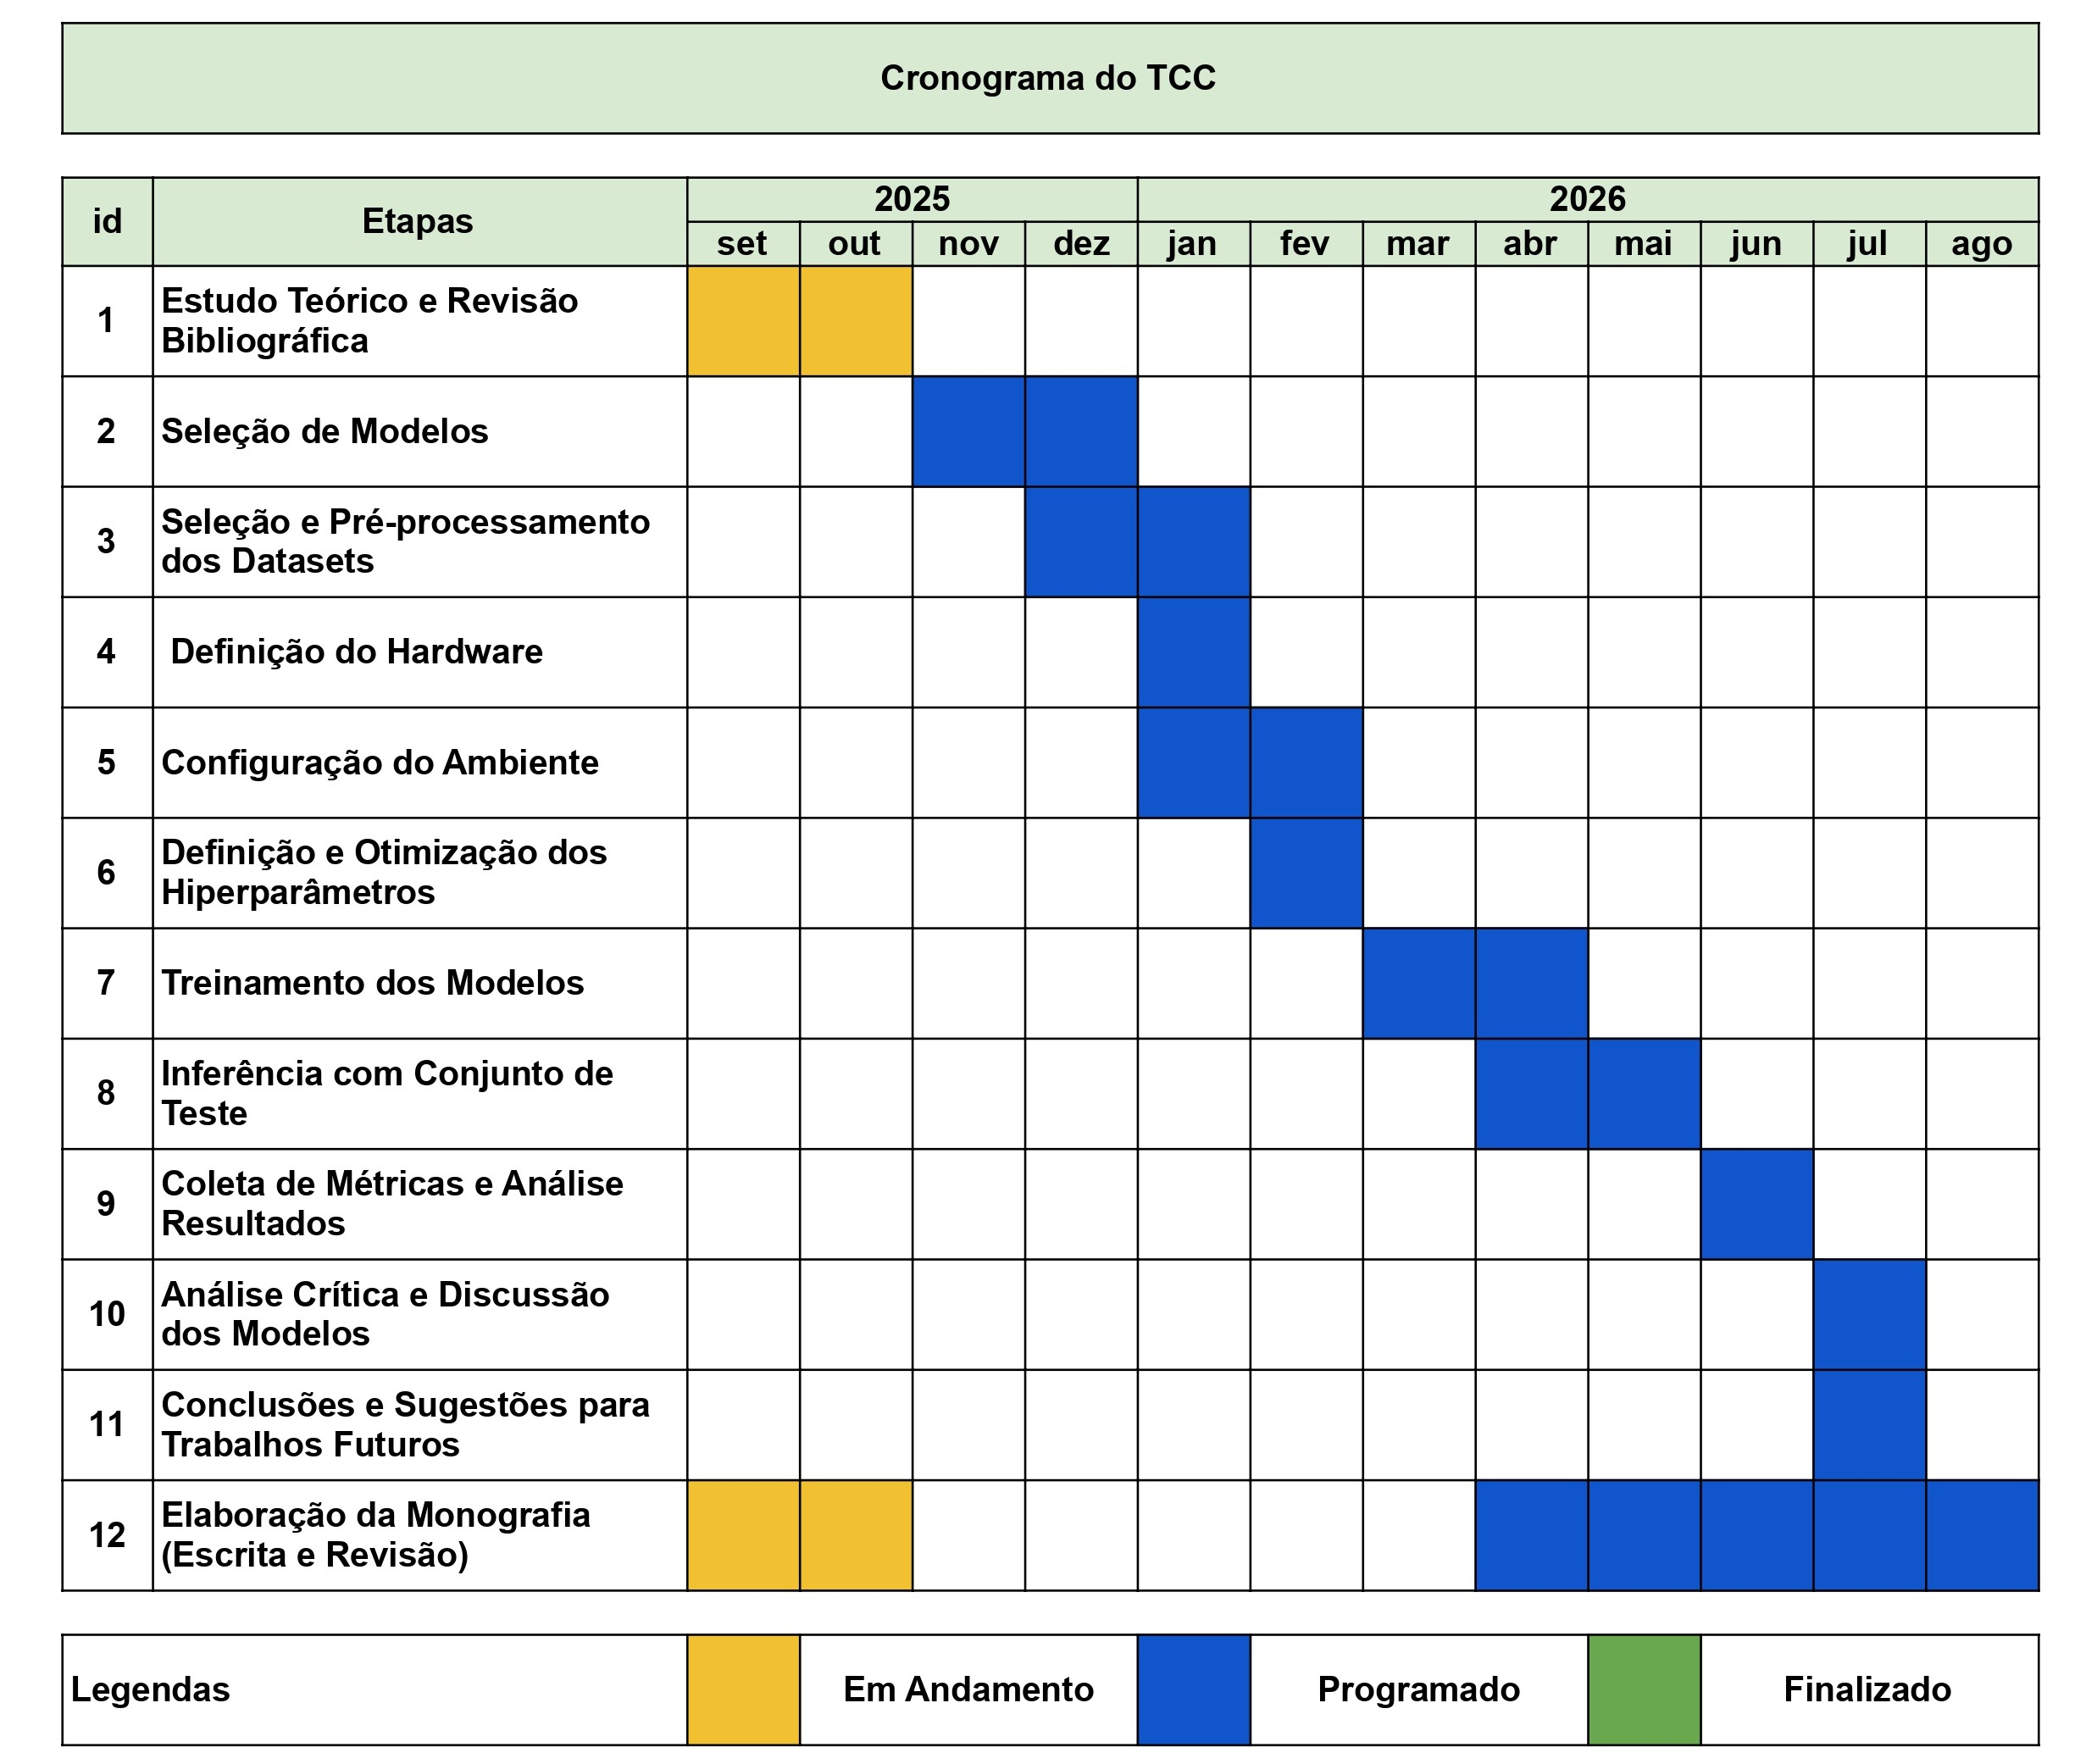
\includegraphics[width=1.0\textwidth]{./media/Cronograma_TCC_Gantt.png}
    \end{Center}
    \label{fig:cronograma}
    \source{Autoria própria (2025).}
\end{figure}

%%%%%%%%%%%%%%%%%%%% Figure/Image Cronograma ends here %%%%%%%%%%%%%%%%%%%%
